\documentclass[../main.tex]{subfiles}
\begin{document}
\chapter{Multivariate Functions: Applications}
\section{Directional Derivatives and Gradient}
Consider $f(x, y)$ and a vector displacement $\d{\vec{s}}=(\d{x}, \d{y})$.
The infinitesimal change in $f$ along $\d{\vec{s}}$ is:
\begin{align*}
  \d{f} &= \pderiv{f}{x}\d{x} + \pderiv{f}{y}\d{y} \\
        &= (\d{x}, \d{y}) \cdot \left(\pderiv{f}{x}, \pderiv{f}{y}\right) \\
        &= \d{\vec{s}} \cdot \nabla f
\end{align*}
where $\nabla f$ is defined as follows.
\begin{definition}[Gradient of $f$]
  The  \textit{gradient of $f$} or grad $f$ is defined to be:
  \[
    \nabla f = \left(\pderiv{f}{x}, \pderiv{f}{y}\right)
  \]
\end{definition}
If we write $\d{\vec{s}} = \d{s}\uvec{s}$, where $\uvec{s}$ is a unit vector, then:
\[
  \d{f} = \d{s}\uvec{s} \cdot \nabla f
\]
\begin{definition}[Directional Derivative]
  The \textit{directional derivative} of $f$ in the direction of $\uvec{s}$ is:
  \[
    \deriv{f}{s} = \uvec{s} \cdot \nabla f
  \]
  where $\uvec{s}$ is a unit vector.
  This tells us the rate of change of $f(x, y)$ in the direction of $\uvec{s}$.
\end{definition}
\begin{center}
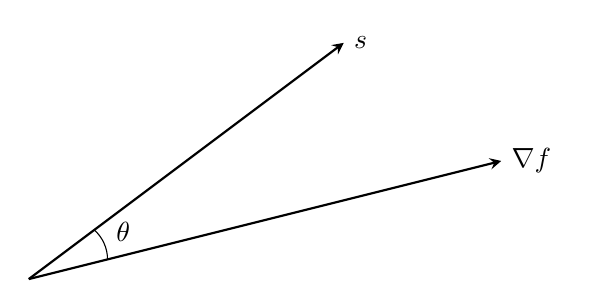
\begin{tikzpicture}[>=stealth, scale=1]
  \draw[->, thick] (0, 0) -- (4, 3) node[right] {$\uvec{s}$};
  \draw[->, thick] (0, 0) -- (6, 1.5) node[right] {$\nabla f$};

  \draw (1,0.25) arc[start angle=0, end angle=49, radius=0.5];

  \node at (1.2,0.6) {$\theta$};
\end{tikzpicture}
\end{center}
Using the definition of the scalar product, we see that:
\[
  \deriv{f}{s} = \uvec{s} \cdot \nabla f = \cos \theta |\nabla f|
\]
\begin{remark}[Note]
  As an alternative, we could have defined $\nabla f$ geometrically as the vector such that:
  \[
    \deriv{f}{s} = \uvec{s} \cdot \nabla f
  \]
  for all $\uvec{s}$.
\end{remark}
\subsection{Properties of the Gradient Vector}
\begin{enumerate}
  \item Direction of $\nabla f$ is that in which $f$ \textbf{increases} most rapidly as the directional derivative is greatest when $\uvec{s}$ is parallel to $\nabla f$
  \item The magnitude of $\nabla f$ is the max rate of change of $f$ at a particular point:
    \[
      |\nabla f| = \max_{\forall \theta}\left(\deriv{f}{s}\right)
    \]
  \item If $\uvec{s}$ is parallel to contours of $f$ (curves of constant $f$), then:
    \[
      \deriv{f}{s} = 0 = \uvec{s} \cdot \nabla f
    \]
    Therefore, $\nabla f$ is perpendicular to the contours of $f$.
\end{enumerate}
\section{Stationary Points}
There is always at least one direction where $\deriv{f}{s} = 0$, i.e. when $\uvec{s}$ is parallel to the contours of $f$.
So to define the notion of a stationary point, we require that $\deriv{f}{s} = 0$ in all directions, not just that $\deriv{f}{s} = 0$ for some $\uvec{s}$.
\begin{definition}[Stationary Point]
  A stationary point is a point where:
  \[
    \deriv{f}{s} = 0\ \forall \uvec{s}
  \]
\end{definition}
So at stationary points:
\[
  \vec{s} \cdot \nabla f = 0\ \forall \uvec{s} \implies \nabla f = \vec{0}
\]
\subsection{Types of Stationary Points}
\label{typesOfStationary}
\subsubsection{Local Maximum}
For a local maximum, $\nabla f$ points towards the maximum point.
Contours are usually locally elliptical around a maximum.
\begin{center}
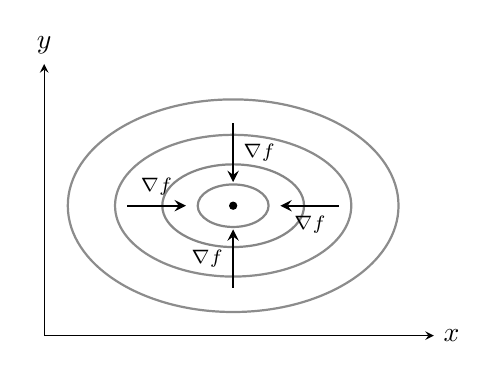
\begin{tikzpicture}[>=stealth, scale=1.5]
\draw[->] (0,0) -- (3.3,0) node[right] {$x$};
\draw[->] (0,0) -- (0,2.3) node[above] {$y$};

\def\cx{1.6}
\def\cy{1.1}

\draw[thick, gray!95] (\cx,\cy) ellipse (0.3 and 0.18);
\draw[thick, gray!95] (\cx,\cy) ellipse (0.6 and 0.35);
\draw[thick, gray!90] (\cx,\cy) ellipse (1.0 and 0.6);
\draw[thick, gray!90] (\cx,\cy) ellipse (1.4 and 0.9);

\fill (\cx,\cy) circle (1pt);

\draw[<-, thick] (\cx,\cy) + (0, -0.2) -- +(0, -0.7) node[midway, left] {$\scriptstyle\nabla f$};
\draw[<-, thick] (\cx,\cy) + (0, 0.2) -- +(0, 0.7) node[midway, right] {$\scriptstyle\nabla f$};
\draw[<-, thick] (\cx,\cy) + (0.4, 0) -- +(0.9, 0) node[midway, below] {$\scriptstyle\nabla f$};
\draw[<-, thick] (\cx,\cy) + (-0.4, 0) -- +(-0.9, 0) node[midway, above] {$\scriptstyle\nabla f$};
\end{tikzpicture}
\end{center}
\subsubsection{Local Minimum}
For a local minimum, $\nabla f$ points away from the minimum point.
Again, contours are usually locally elliptical.
\begin{center}
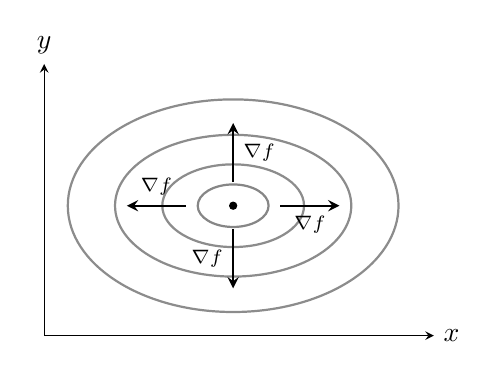
\begin{tikzpicture}[>=stealth, scale=1.5]
\draw[->] (0,0) -- (3.3,0) node[right] {$x$};
\draw[->] (0,0) -- (0,2.3) node[above] {$y$};

\def\cx{1.6}
\def\cy{1.1}

\draw[thick, gray!95] (\cx,\cy) ellipse (0.3 and 0.18);
\draw[thick, gray!90] (\cx,\cy) ellipse (0.6 and 0.35);
\draw[thick, gray!90] (\cx,\cy) ellipse (1.0 and 0.6);
\draw[thick, gray!90] (\cx,\cy) ellipse (1.4 and 0.9);

\fill (\cx,\cy) circle (1pt);

\draw[->, thick] (\cx,\cy) + (0, -0.2) -- +(0, -0.7) node[midway, left] {$\scriptstyle\nabla f$};
\draw[->, thick] (\cx,\cy) + (0, 0.2) -- +(0, 0.7) node[midway, right] {$\scriptstyle\nabla f$};
\draw[->, thick] (\cx,\cy) + (0.4, 0) -- +(0.9, 0) node[midway, below] {$\scriptstyle\nabla f$};
\draw[->, thick] (\cx,\cy) + (-0.4, 0) -- +(-0.9, 0) node[midway, above] {$\scriptstyle\nabla f$};
\end{tikzpicture}
\end{center}
\subsubsection{Saddle Point}
A saddle point is \textbf{not} a local extremum.
Generally speaking, in one direction it is a maximum and in another direction it is a minimum.
Contours always cross and only ever cross at a saddle points.
Around a saddle point, the contours are usually locally hyperbolic.
\begin{center}
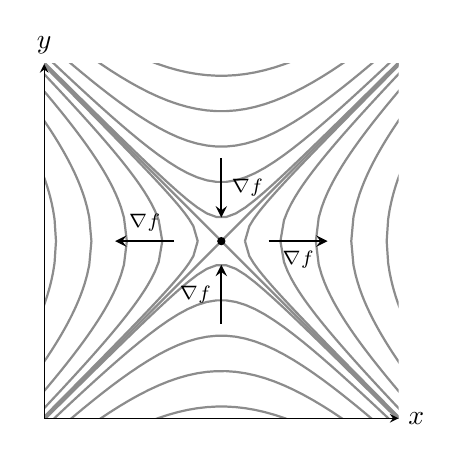
\begin{tikzpicture}[scale=1.5, >=stealth]
\def\cx{1.5}
\def\cy{1.5}
\begin{scope}
\clip (0, 0) rectangle (3, 3);
\foreach \b in {0.2, 0.5, 0.8, 1.1, 1.4}{
    \draw[thick, gray!90, domain=\cx+\b:\cx+2, samples=50] plot ({\x}, {\cy + sqrt((\x-\cx)^2 - \b^2)});
    \draw[thick, gray!90, domain=\cx+\b:\cx+2, samples=50] plot ({\x}, {\cy - sqrt((\x-\cx)^2 - \b^2)});
    \begin{scope}[xscale=-1, xshift=-3cm]
      \draw[thick, gray!90, domain=\cx+\b:\cx+2, samples=50] plot ({\x}, {\cy + sqrt((\x-\cx)^2 - \b^2)});
      \draw[thick, gray!90, domain=\cx+\b:\cx+2, samples=50] plot ({\x}, {\cy - sqrt((\x-\cx)^2 - \b^2)});
    \end{scope}
    \draw[thick, gray!90, domain=\cx-2:\cx+2, samples=50] plot ({\x}, {\cy + sqrt((\x-\cx)^2 + \b^2)});
    \draw[thick, gray!90, domain=\cx-2:\cx+2, samples=50] plot ({\x}, {\cy - sqrt((\x-\cx)^2 + \b^2)});
}
\draw[thick, gray!90] (\cx, \cy) + (-2, -2) -- +(2, 2);
\draw[thick, gray!90] (\cx, \cy) + (2, -2) -- +(-2, 2);
\end{scope}

\fill (\cx,\cy) circle (1pt);
\draw[<-, thick] (\cx,\cy) + (0, -0.2) -- +(0, -0.7) node[midway, left] {$\scriptstyle\nabla f$};
\draw[<-, thick] (\cx,\cy) + (0, 0.2) -- +(0, 0.7) node[midway, right] {$\scriptstyle\nabla f$};
\draw[->, thick] (\cx,\cy) + (0.4, 0) -- +(0.9, 0) node[midway, below] {$\scriptstyle\nabla f$};
\draw[->, thick] (\cx,\cy) + (-0.4, 0) -- +(-0.9, 0) node[midway, above] {$\scriptstyle\nabla f$};

\draw[->] (0,0) -- (3,0) node[right] {$x$};
\draw[->] (0,0) -- (0,3) node[above] {$y$};
\end{tikzpicture}
\end{center}
\section{Classification of Stationary Points}
How does $f$ change in the vicinity of a stationary point?
\subsection{Taylor Series for Multivariate Functions}
Consider how $f(x, y)$ varies along the line $\vec{x}(s) = \vec{x}_0 + s \uvec{s}$.
\begin{center}
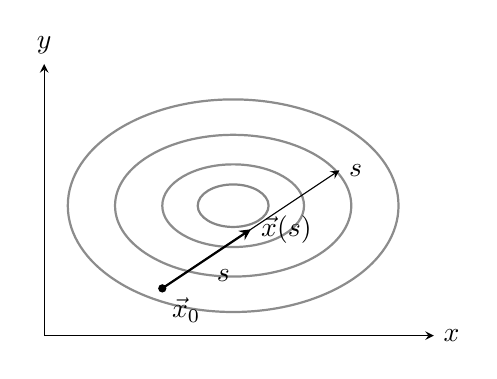
\begin{tikzpicture}[>=stealth, scale=1.5]
\draw[->] (0,0) -- (3.3,0) node[right] {$x$};
\draw[->] (0,0) -- (0,2.3) node[above] {$y$};

\def\cx{1.6}
\def\cy{1.1}

\draw[thick, gray!95] (\cx,\cy) ellipse (0.3 and 0.18);
\draw[thick, gray!90] (\cx,\cy) ellipse (0.6 and 0.35);
\draw[thick, gray!90] (\cx,\cy) ellipse (1.0 and 0.6);
\draw[thick, gray!90] (\cx,\cy) ellipse (1.4 and 0.9);

\coordinate (X) at (1, 0.4);
\fill (X) circle (1pt) node[below right] {$\vec{x}_0$};
\draw[->] (X) -- +(1.5, 1) node[right] {$\uvec{s}$};
\draw[->, thick] (X) -- +(0.75, 0.5) node[right] {$\vec{x}(s)$} node[midway, below right] {$s$};
\end{tikzpicture}
\end{center}
Along this line, $f(\vec{x}_0 + s \uvec{s}) = f(x(s), y(s))$ so $f$ is a function of $s$.
Therefore, we can use the usual Taylor series:
\begin{align*}
  f(\vec{x}_0 + s \uvec{s}) &= f(\vec{x}_0) + s \at{\deriv{f}{s}}{\vec{x}_0} + \frac{1}{2}s^2 \at{\deriv[2]{f}{s}}{\vec{x}_0} + \cdots \\
                            &= f(\vec{x}_0) + s \uvec{s} \cdot \at{\nabla f}{\vec{x}_0} + \frac{1}{2}s^2 \at{(\uvec{s} \cdot \nabla)(\uvec{s} \cdot \nabla f)}{\vec{x}_0} + \cdots
\end{align*}
Looking at the second term of the expansion, let $\delta\vec{x} = (x - x_0, y - y_0) = (\delta x, \delta y) = s \uvec{s}$.
We then have:
\[
  s \uvec{s} \cdot \nabla f = \delta \vec{x} \cdot \nabla f = \delta x \pderiv{f}{x} + \delta y \pderiv{f}{y}
\]
Looking at the third term of the expansion, let $\hat{s}_x$ and $\hat{s}_y$ be the components of $\uvec{s} =(\hat{s}_x, \hat{s}_y)$.
We then have:
\begin{align*}
  s^2(\uvec{s} \cdot \nabla)(\uvec{s} \cdot \nabla f) &= s^2\left(\hat{s}_x \pderiv{}{x} + \hat{s}_y \pderiv{}{y}\right)\left(\hat{s}_x \pderiv{f}{x} + \hat{s}_y \pderiv{f}{y}\right) \\
                                                      &= \left(\delta x \pderiv{}{x} + \delta y \pderiv{}{y}\right)\left(\delta x \pderiv{f}{x} + \delta y \pderiv{f}{y}\right) \\
                                                      &= (\delta x)^2 \pderiv[2]{f}{x} + (\delta x)(\delta y) \frac{\partial^2 f}{\partial x \partial y} + (\delta y)(\delta x)\frac{\partial^2 f}{\partial y \partial x} + (\delta y)^2 \pderiv[2]{f}{y} \\
                                                      &= (\delta x, \delta y)
                                                      \begin{pmatrix}
                                                      f_{x x} & f_{x y} \\
                                                      f_{y x} & f_{y y} \\
                                                      \end{pmatrix}
                                                      \begin{pmatrix}
                                                      \delta x \\
                                                      \delta y \\
                                                      \end{pmatrix}
\end{align*}
\begin{definition}[Hessian Matrix]
  The \textit{Hessian Matrix} is defined to be:
  \[
    H = \nabla \nabla f = \begin{pmatrix}
    f_{x x} & f_{x y} \\
    f_{y x} & f_{y y} \\
    \end{pmatrix}
  \]
  This is symmetric as $f_{x y} = f_{y x}$.
\end{definition}
The multivariate Taylor series is then:
\begin{align*}
  f(x_0 + \delta x, y_0 + \delta y) &= f(x_0, y_0) + \at{\left[\delta x \pderiv{f}{x} + \delta y \pderiv{f}{y}\right]}{(x_0, y_0)} \\ &\quad+\frac{1}{2}\at{\left[(\delta x)^2 \pderiv[2]{f}{x} + 2\delta x\delta y \frac{\partial^2 f}{\partial x \partial y} + (\delta y)^2 \pderiv[2]{f}{y}\right]}{(x_0, y_0)} + \cdots
\end{align*}
This can be written in a coordinate independent form as:
\begin{align*}
  f(\vec{x}_0 + \delta \vec{x}) &= f(\vec{x}_0) + \delta \vec{x} \cdot \at{(\nabla f)}{\vec{x}_0} + \frac{1}{2} (\delta \vec{x})^{\trans} \at{H}{\vec{x}_0} \delta \vec{x} + \cdots \\
                                & =f(\vec{x}_0) + \delta \vec{x} \cdot \at{(\nabla f)}{\vec{x}_0} + \frac{1}{2} (\delta \vec{x})^{\trans} \at{(\nabla \nabla f)}{\vec{x}_0} \delta \vec{x} + \cdots
\end{align*}
\subsection{Classification of Stationary Points}
Suppose $\vec{x}_0$ is a stationary point, that is $\at{\nabla f}{\vec{x}_0} = \vec{0}$.

Using the multivariate Taylor series, around $\vec{x}_0$ we have:
\[
  f(\vec{x}) \approx f(\vec{x}_0) + \frac{1}{2} (\delta \vec{x})^{\trans} H (\delta\vec{x})
\]
where $\delta \vec{x} = \vec{x} - \vec{x}_0$.
\begin{definition}[Positive and Negative Definite]
  A real symmetric matrix $H$ is:
  \begin{itemize}
    \item \textit{Positive definite}, if:
      \[
        \vec{x}^{\trans} H \vec{x} > 0\ \forall \vec{x} \in \R^{n}, \vec{x} \neq \vec{0}
      \]
    \item \textit{Negative definite}, if:
      \[
        \vec{x}^{\trans} H \vec{x} < 0\ \forall \vec{x} \in \R^{n}, \vec{x} \neq \vec{0}
      \]
    \item \textit{Indefinite} otherwise.
  \end{itemize}
\end{definition}
\begin{itemize}
  \item If $H$ is \textbf{positive definite} at $\vec{x}_0$, then the stationary point is a local minimum as $f(\vec{x}) > f(\vec{x}_0)$ close to $\vec{x}_0$.
  \item If $H$ is \textbf{negative definite} at $\vec{x}_0$, then the stationary point is a local maximum as $f(\vec{x}) < f(\vec{x}_0)$ close to $\vec{x}_0$.
  \item If $H$ is \textbf{indefinite}, then the stationary point may be a maximum, minimum or a saddle point.
\end{itemize}
\subsection{Definiteness and Eigenvalues}
$H$ is a real symmetric matrix, therefore it can be diagonalised with an orthogonal transformation. This corresponds to using coordinates along the principal axes (that is, the axes defined by the eigenvectors).
\textit{(For more details see Vectors and Matrices 4.6)}

After diagonalisation, in $n$ dimensions:
\begin{align*}
  (\delta \vec{x})^{\trans}H(\delta\vec{x}) &= (\delta x_1, \ldots, \delta x_n)
  \begin{pmatrix}
  \lambda_1 &  &  \\
   & \ddots &  \\
   &  & \lambda_n \\
  \end{pmatrix}
  \begin{pmatrix}
  \delta x_1 \\
  \vdots \\
  \delta x_n \\
  \end{pmatrix} \\
  &= \lambda_1 (\delta x_1)^2 + \lambda_2 (\delta x_2)^2 + \cdots + \lambda_n(\delta x_n)^2
\end{align*}
where $\delta x_i$ are the coordinates with respect to the principal axes.

Since the definiteness of $H$ depends on whether the relation holds for all $\delta \vec{x}$, we can conclude that:
\begin{itemize}
  \item $H$ is \textbf{positive definite} if and only if all $\lambda_i > 0$ $\to$ \textbf{Minimum} point.
  \item $H$ is \textbf{negative definite} if and only if all $\lambda_i < 0$ $\to$ \textbf{Maximum} point.
  \item All eigenvalues are \textbf{non-zero and mixed signs} $\to$ \textbf{Saddle} point.
  \item \textbf{Any} eigenvalues are 0 $\to$ Need higher order terms in the Taylor series to classify the stationary point.
\end{itemize}
\begin{example}
  \[
    f(x, y) = x^2 + y^4
  \]
  We can see that is has a global minimum at $(0, 0)$.
  First we find $\nabla f$:
  \[
    \nabla f = (f_x, f_y) = (2x, 4y^3)
  \]
  We then can find the Hessian at $(0, 0)$:
  \[
    H = \begin{pmatrix}
    2 & 0 \\
    0 & 12y^2 \\
    \end{pmatrix} \implies
    \at{H}{(0, 0)} =
    \begin{pmatrix}
    2 & 0 \\
    0 & 0 \\
    \end{pmatrix}
  \]
  which has eigenvalues $\lambda_1 = 2$ and $\lambda_2 = 0$.
  Since one of the eigenvalues is 0, we would need to use higher order terms in the Taylor series to classify the stationary point using this method.
\end{example}
\subsection{Definiteness and Signature}
The signature of the Hessian matrix provides an alternative method for classifying stationary points that does not involve computing eigenvalues.

\begin{definition}[Signature]
  The \textit{signature} of $H$ is the pattern of signs of the ordered sub-determinants of the leading principal minors of $H$.
\end{definition}
For $f(x_1, x_2, \ldots, x_n)$, the sub-determinants of the leading principal minors of $H$ are:
\begin{align*}
  |H_1| &= |f_{x_1 x_1}| \\
  |H_2| &= \begin{vmatrix}
  f_{x_1 x_1} & f_{x_1 x_2} \\
  f_{x_2 x_1} & f_{x_2 x_2} \\
  \end{vmatrix} \\
  &\ \ \vdots \\
  |H_n| &= \begin{vmatrix}
  f_{x_1 x_1} & \cdots & f_{x_1 x_n} \\
  \vdots & \ddots & \vdots \\
  f_{x_n x_1} & \cdots & f_{x_nx_n } \\
  \end{vmatrix}
\end{align*}
So the signature of $H$ is: sign of $|H_1|$, sign of $|H_2|$, ..., sign of $|H_n|$.
\begin{theorem}[Slyvesters Critereon]
  \label{syvestersCritereon}
  For a symmetric matrix $H$:
  \begin{align*}
    H \text{ is positive definite} &\iff \text{ signature is: }+, +, +, \cdots, +\\
    H \text{ is negative definite} &\iff \text{ signature is: }-, +, -, +, \cdots
  \end{align*}
  If $H$ has any other signature, it is indefinite.
\end{theorem}
\subsection{Contours Near Stationary Points}
Suppose $f(x, y)$ has a stationary point at $\vec{x}_0 = (x_0, y_0)$.
For ease, use the coordinates aligned with the principal axes of $H(\vec{x}_0)$.
So $H(\vec{x}_0)$ will be diagonal:
\[
  H(\vec{x}_0) = \begin{pmatrix}
  \lambda_1 & 0 \\
  0 & \lambda_2 \\
  \end{pmatrix}
\]
We are going to assume the eigenvalues are non-zero for simplicity.
Consider $\delta \vec{x} = (\xi, \eta)$ for small $\xi$ and $\eta$.
\[
  \vec{x} = \vec{x}_0 + (\xi, \eta)
\]
Then around $\vec{x}_0$ we  have:
\[
  f(\vec{x}) = f(\vec{x}_0) + \frac{1}{2}(\lambda_1 \xi^2 + \lambda_2 \eta^2) + \cdots
\]
Close to $\vec{x}_0$, the higher order terms become negligible.
Therefore, close to $\vec{x}_0$ the contours have the form:
\[
  \lambda_1 \xi^2 + \lambda_2 \eta^2 = \text{constant}
\]
For a maximum or minimum, both eigenvalues share the same sign so we see that this describes an ellipse with respect to the principal axes of $H(\vec{x}_0)$.

At  a saddle point, the eigenvalues have opposite signs so we see that describes a hyperbola with respect to the principal axes of $H(\vec{x}_0)$.

This agrees with what we saw in \cref{typesOfStationary}.
\subsection{Example of Classifying Stationary Points}
\begin{example}
  Find and classify the stationary points of:
  \[
    f(x, y) = 4x^3 - 12xy + y^2 + 10y+ 6
  \]
  \begin{align*}
    \nabla f = (f_x, f_y) = (12x^2 - 12y, -12x + 2y + 10)
  \end{align*}
  We have stationary points when both $f_x$ and $f_y$ are 0.
  \begin{align*}
    f_x &= 0 \implies y = x^2 \\
    f_y &= 0 \implies -12x + 2y + 10 = 0
  \end{align*}
  Combining the above we have:
  \begin{align*}
    -12x + 2x^2 + 10 &= 0 \\
    x^2 - 6x + 5 &= 0
  \end{align*}
  This has roots at $x = 1$ and $x = 5$.
  Therefore the stationary points are at $(1, 1)$ and $(5, 25)$.

  Now to compute the Hessian we first find:
  \[
    f_{x x} = 24x,\ f_{x y} = -12,\ f_{y y} = 2
  \]
  So:
  \[
    H = \begin{pmatrix}
    24x & -12 \\
    -12 & 2 \\
    \end{pmatrix}
  \]
  First, considering the stationary point $(1, 1)$:
  \[
    \at{H}{(1, 1)} = \begin{pmatrix}
    24 & -12 \\
    -12 & 2 \\
    \end{pmatrix}
  \]
  So $|H_1| = 24$ and $|H_2| = -96$.
  So the signature is $+, -$ which doesn't match either of the conditions in \cref{syvestersCritereon}, thus $H$ is indefinite.
  Since the diagonalised form of $H$ has the same determinant and $|H| \neq 0$, the product of all eigenvalues is non-zero.
  Therefore, all eigenvalues are non-zero and have mixed signs so we have a saddle point.

  Now, considering the stationary point $(5, 25)$
  \[
    \at{H}{(5, 25)} = \begin{pmatrix}
    120 & -12 \\
    -12 & 2 \\
    \end{pmatrix}
  \]
  So $|H_1| = 120$ and $|H_2| = 240 - 144 = 96$.
  So the signature is $+, +$, so we see from \cref{syvestersCritereon} that $H$ is positive definite.
  Therefore we have a local minimum.

  Near the saddle point, the contours satisfy
  \[
    24(\delta x)^2 - 24(\delta x)(\delta y) + 2(\delta y)^2 = \text{constant}
  \]
  If we find the eigenvalues and eigenvectors of $\at{H}{(5, 25)}$, this will define an ellipse aligned with the principal axes of $\at{H}{(5, 25)}$.

\textit{(For more details see Vectors and Matrices 4.6)}
\end{example}
\end{document}
